% !TEX root =../LibroTipoETSI.tex
\section{Pruebas realizadas}\label{sec:pruebas}
\subsection{Pruebas de laboratorio}
\subsubsection{Entorno del laboratorio}

El equipo \gls{DUT} es un redBorder IPS de 8 hilos (1 quad-core de 2 hilos por core) Intel Xeon E3-1240 a 3.30GHz. La 
interfaz del segmento de inspección es una intel quad-ethernet 82580 Gigabit con soporte bypass. En el sensor se ha 
instalado la distribución \emph{redBorder-IPS-sensor 3.0.30-1}, basada en la distribución Linux CentOS 6.5.

Como generador de tráfico, se usará otro dispositivo con las mismas características. Los segmentos de $1G$ se unirán de 
un equipo a otro en el mismo orden, a fin de facilitar el entendimiento de las pruebas, y serán llamados 
\text{eth4}, \text{eth5}, \text{eth6}, y \text{eth7} de izquierda a derecha.

Se dispone, además de una captura de tráfico llamada \emph{entrenamiento.pcap}, que contiene tráfico real sin ataques,
y que reproduciremos gracias al comando \texttt{tcpreplay}.

\subsubsection{Prueba 1: Ajuste de los parámetros CUSUM para evitar falsos positivos}
\paragraph{Descripción de la prueba}\mbox{}

El primer paso de cara a realizar las pruebas es conseguir un valor adecuado del número de desviaciones límites
para tener en cuenta la medida y para generar una alarma.

\paragraph{Procedimiento}\mbox{}

Con un PCAP concreto, se debe realizar un periodo de aprendizaje. Tras él, se debe realizar un
periodo de defensa con el mismo PCAP y los valores límites propuestos. Si éstos generan alertas,
significa que esos valores son extremadamente bajos.

\paragraph{Resultados}\mbox{}

Como valores iniciales, se escogieron los recomendados por Ismael Sánchez, $C_i^+=5$ y $C_i^{min}=2.5$
 \cite{CUSUM_Carlos_III}.

Tras realizar las pruebas, se observó que la naturaleza de la red de datos, en el que el tráfico suele ser la 
mayor parte del tiempo $0$ y, durante un breve intervalo de tiempo, un valor elevado, provocaban que fuese necesario
el aumento de esos valores iniciales, que finalmente fueron establecidos a $C_i^+=10$ y $C_i^{min}=5$. Esto fue
especialmente influyente en el tráfico \gls{ICMP}, por lo que se decidió no tenerlo en cuenta para generar alarmas.

\subsubsection{Prueba 2: Detección de IPs atacantes, control de falsos negativos y estado de 
alerta}
\paragraph{Descripción de la prueba}\mbox{}

Con el aprendizaje de la prueba anterior, se hará pasar 
la captura \emph{entrenamiento.pcap} y, al cabo de un tiempo $T_0$, 
se pasará una ráfaga de paquetes UDP a alta velocidad (ataque), desde un pcap preparado.

Tras ello, se analiza la salida, en busca de:
\begin{itemize}
 \item Número de paquetes analizados por el programa.
 \item Si el programa ha estado en alerta o no.
\end{itemize}

%TODO corregir ortografía "Resultados", "bajo", en pfc
\paragraph{Resultados}\mbox{}

En los resultados, \texttt{rbddos} fue capaz de marcar los momentos bajo ataque a distintas velocidades, y todos los 
elementos atacantes pertenecían al conjunto de direcciones IP correctos.

\subsection{Prueba realizada en Produban}
\subsubsection{Contexto}
El día 4 de mayo de 2013, Produbán, empresa de gestión IT del grupo Santanter, pidió a Eneo un sistema que de detección 
de ataques \gls{DDoS}, dado que tenía la sospecha de que se iba a producir un ataque real a su infraestructura.

Pese a estar aún en un estado muy prematuro, Produban aceptó la instalación del software ya que no entrañaba riesgo 
para la infraestructura al estar este situado en un puerto SPAN.

\begin{figure}[hbtp]
  \centering
  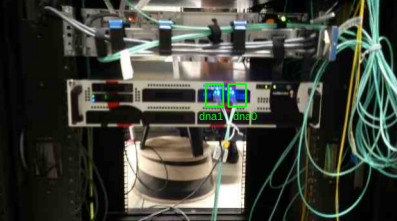
\includegraphics[width=\columnwidth]{CapituloPruebas/Figuras/ProdubanFrontal}
  \caption{Parte frontal del sensor}
  \label{fig:produban_mesena_frontal}
\end{figure}
\begin{figure}[hbtp]
  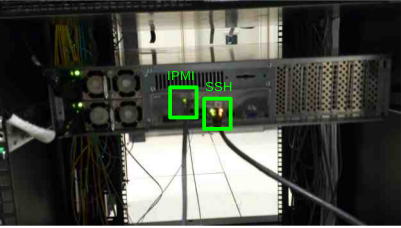
\includegraphics[width=\columnwidth]{CapituloPruebas/Figuras/ProdubanTrasera}
  \caption{Parte trasera del sensor}
  \label{fig:produban_mesena_trasera}
\caption{Instalación de \redborderddos{} en el CPD de Mesena, Produban}
\end{figure}
%

El sensor usado es un equipo 2U con doble procesador Xeon E5 y 64GB de RAM, con 2 puertos dedicados de gestión y otros 
2 puertos 10G para conectarse a un puerto de SPAN, y es instalado en el CPD de Mesena. Vemos su parte frontal y
en la \autoref{fig:produban_mesena_frontal}, con sus puertos de inspección, y la parte trasera en
\autoref{fig:produban_mesena_trasera}, con su interfaz de gestión e IPMI.


\subsubsection{Resultados}
Debido a lo inmediato de la instalación, fue imposible ajustar el sensor para que diese resultados significativos. Con 
sólo tres horas de entrenamiento, y sin ser estas siquiera determinantes, era muy difícil que la prueba diese 
resultados satisfactorios. El programa estuvo ejecutándose desde el 7 de mayo a las 
11:53\footnote{Timestamp: 1367920409} hasta el 15 de mayo a las 11:36, y se generaron más de 100 millones de alarmas.

Las conclusiones principales que se extrayeron fue que la realidad era mucho más cambiante de lo que permitía discernir 
tres horas de entrenamiento, o incluso un día, y que se debería de adaptar el protocolo CUSUM para hacer frente a esa 
realidad.

\endinput
